\documentclass{beamer}
\usepackage{animate}
\usepackage{graphics}
\usepackage{amsmath}
\usepackage{hyperref}
\usepackage{listings}  % Include the listings package for code
\usetheme[sectionpage=none, progressbar=frametitle, numbering=fraction]{metropolis}  % Use metropolis theme  
\usetheme[sectionpage=none, progressbar=frametitle, numbering=fraction]{metropolis}  % Use metropolis theme  
\title{Mathematik in der Spielentwicklung}
\date{}
\author{Mikhail Safonov}  % Remove if not needed
\institute{}  % Remove if not needed



\usepackage[utf8]{inputenc}  % Add this for UTF-8 encoding support

\setbeamertemplate{title separator}{\vskip0.2cm\hrule height 0.5pt width \linewidth\hspace{0.2cm}\vskip0.3cm}  
\setbeamercolor{title separator}{fg=orange}  % Set color for title separator

\titlegraphic{\includegraphics[width=0.3\textwidth]{bilder/HsH.png}} 

\begin{document}
	
	\maketitle
	
\begin{frame}
	\frametitle{Gliederung}
	\centering
	\begin{minipage}{0.5\textwidth}
		\centering
		\rotatebox{90}{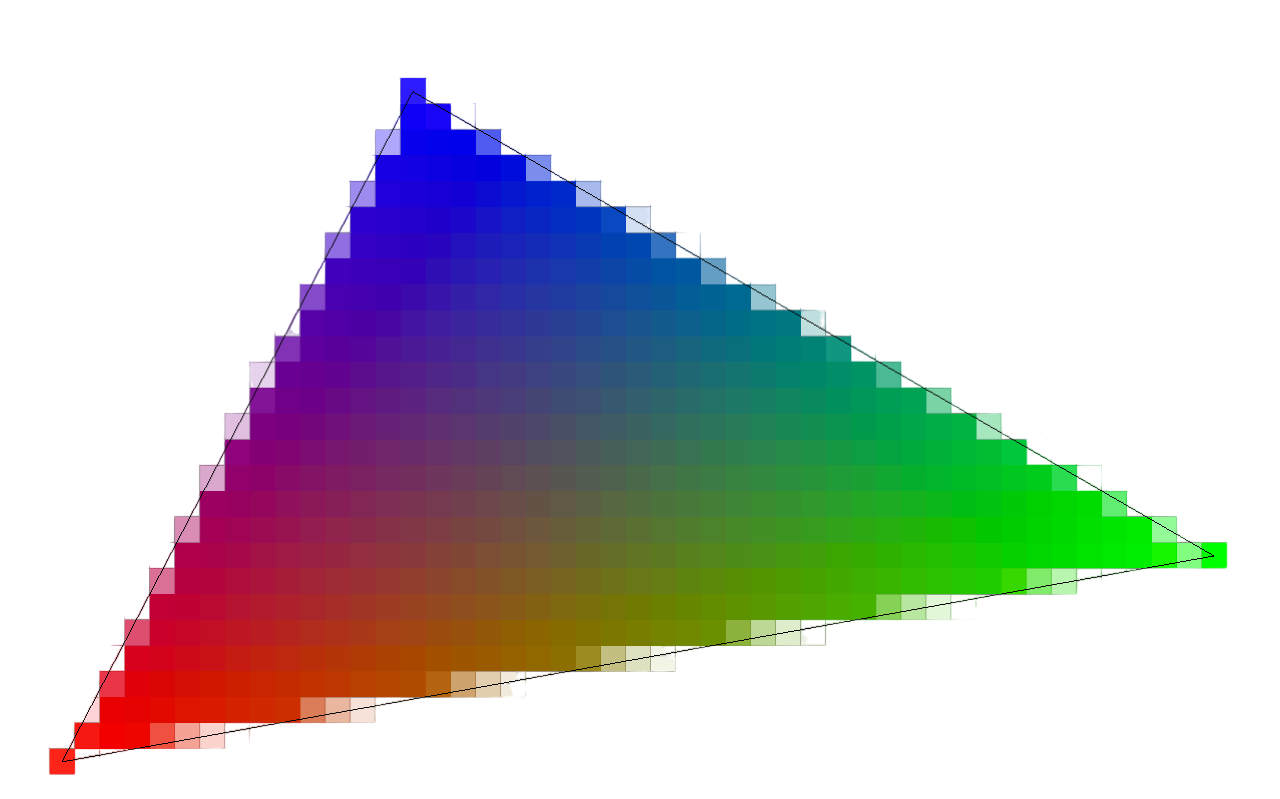
\includegraphics[width=7cm]{bilder/ii-.png}}
	\end{minipage}%
	\begin{minipage}{0.45\textwidth}
		\begin{itemize}
			\small
			\item Triangulation
			\item Rasterung
			\item Raytraycing
			\item Baryzentrische Koordinaten
			\item Rotation
		\end{itemize}
	\end{minipage}
\end{frame}

\begin{frame}
	\frametitle{Triangulation}
	\vspace{0.5cm}
	\textmd{\small Warum gerade Dreiecke? Aus Dreiecken können alle anderen Vielecke zusammengesetzt werden, und Dreiecke lassen sich besonders einfach mit dem Computer zeichnen. Das Problem, ein komplexes 3D-Objekt wie zum Beispiel ein Flugzeug zu zeichnen, kann also auf das Problem reduziert werden, viele Dreiecke zu zeichnen.} \\
	\vspace{0.3cm} % Adjust spacing between text and image
	\centering
	
\includegraphics[width=10cm]{bilder/triangles-.png}
	
\end{frame}

\begin{frame}
	\frametitle{\phantom{}}
	\vspace{0.5cm}
	\centering
	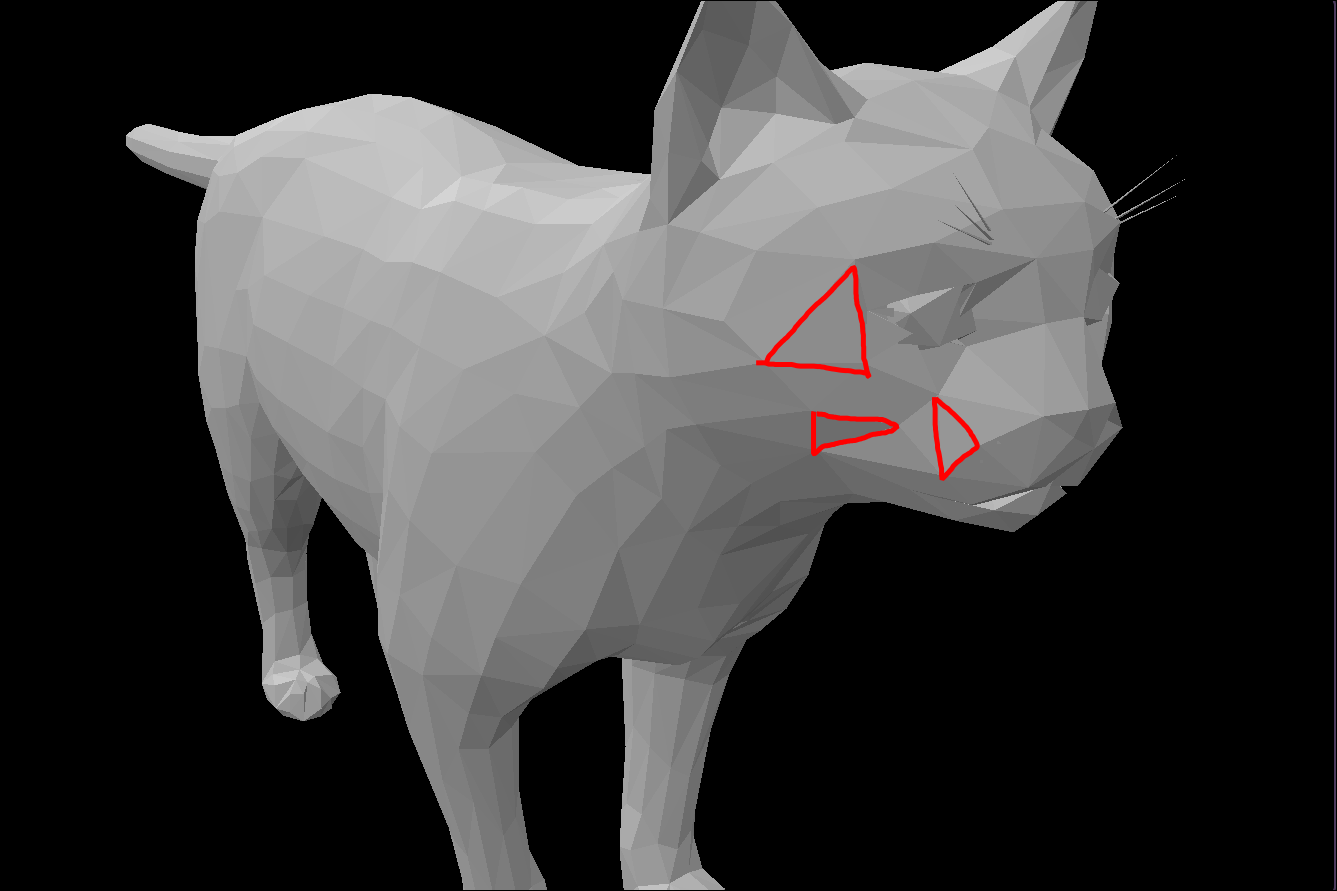
\includegraphics[width=10cm]{bilder/cat.png}
\end{frame}


\begin{frame}
	\frametitle{Rasterung}
		\vspace{0.5cm}
		\textmd{\small Bei Rasterung werden die darzustellenden Dreiecke gerastert, also auf diskrete Bildpunkte abgebildet. Ein Dreieck kann man dann zeichnen und ausfüllen, indem man es Zeile für Zeile von oben nach unten abläuft und jede Zeile füllt. Eine Zeile entspricht dabei einer Pixelzeile. Dieses Verfahren, das heutige Grafikkarten anwenden, nennt man Scanline Rendering.} \\
		\vspace{0.3cm} % Adjust spacing between text and image
		\centering
		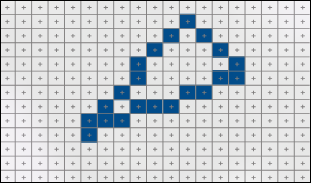
\includegraphics[width=5cm]{bilder/scan-.png}
\end{frame}

\begin{frame}
	\frametitle{\phantom{}}
	\vspace{0.5cm}
	\textmd{\small Bei Rasterung werden die darzustellenden Dreiecke gerastert, also auf diskrete Bildpunkte abgebildet. Ein Dreieck kann man dann zeichnen und ausfüllen, indem man es Zeile für Zeile von oben nach unten abläuft und jede Zeile füllt. Eine Zeile entspricht dabei einer Pixelzeile. Dieses Verfahren, das heutige Grafikkarten anwenden, nennt man Scanline Rendering.} \\
	\vspace{0.3cm} % Adjust spacing between text and image
	\centering
	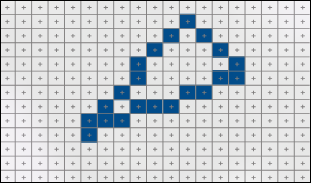
\includegraphics[width=5cm]{bilder/scan-.png}
	\hspace{0.05\textwidth}
	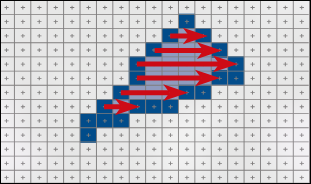
\includegraphics[width=5cm]{bilder/scan.png}
\end{frame}

\begin{frame}
		\frametitle{Raytracing}
		\textmd{\small
			Raytracing wird, vereinfacht gesagt, für jeden Pixel des Bildes ein virtueller Strahl (Sichtstrahl) in die Szene geschossen, und es wird berechnet, ob er ein Objekt schneidet. Wenn das der Fall ist, wird der Pixel entsprechend eingefärbt.
		}
		
		\vspace{0.3cm}
		Raytracing-Verfahren:
		\begin{itemize}
			\item {\small liefern Bilder von sehr hoher Qualität} 
			\item {\small sind generell sehr flexibel} 
			\item {\small sowohl mit mathematischer Darstellungsweise von 3D-Szenen als auch mit triangulierten Objekten}
		\end{itemize}
\end{frame}

\begin{frame}
	\frametitle{\phantom{}}
	\centering
	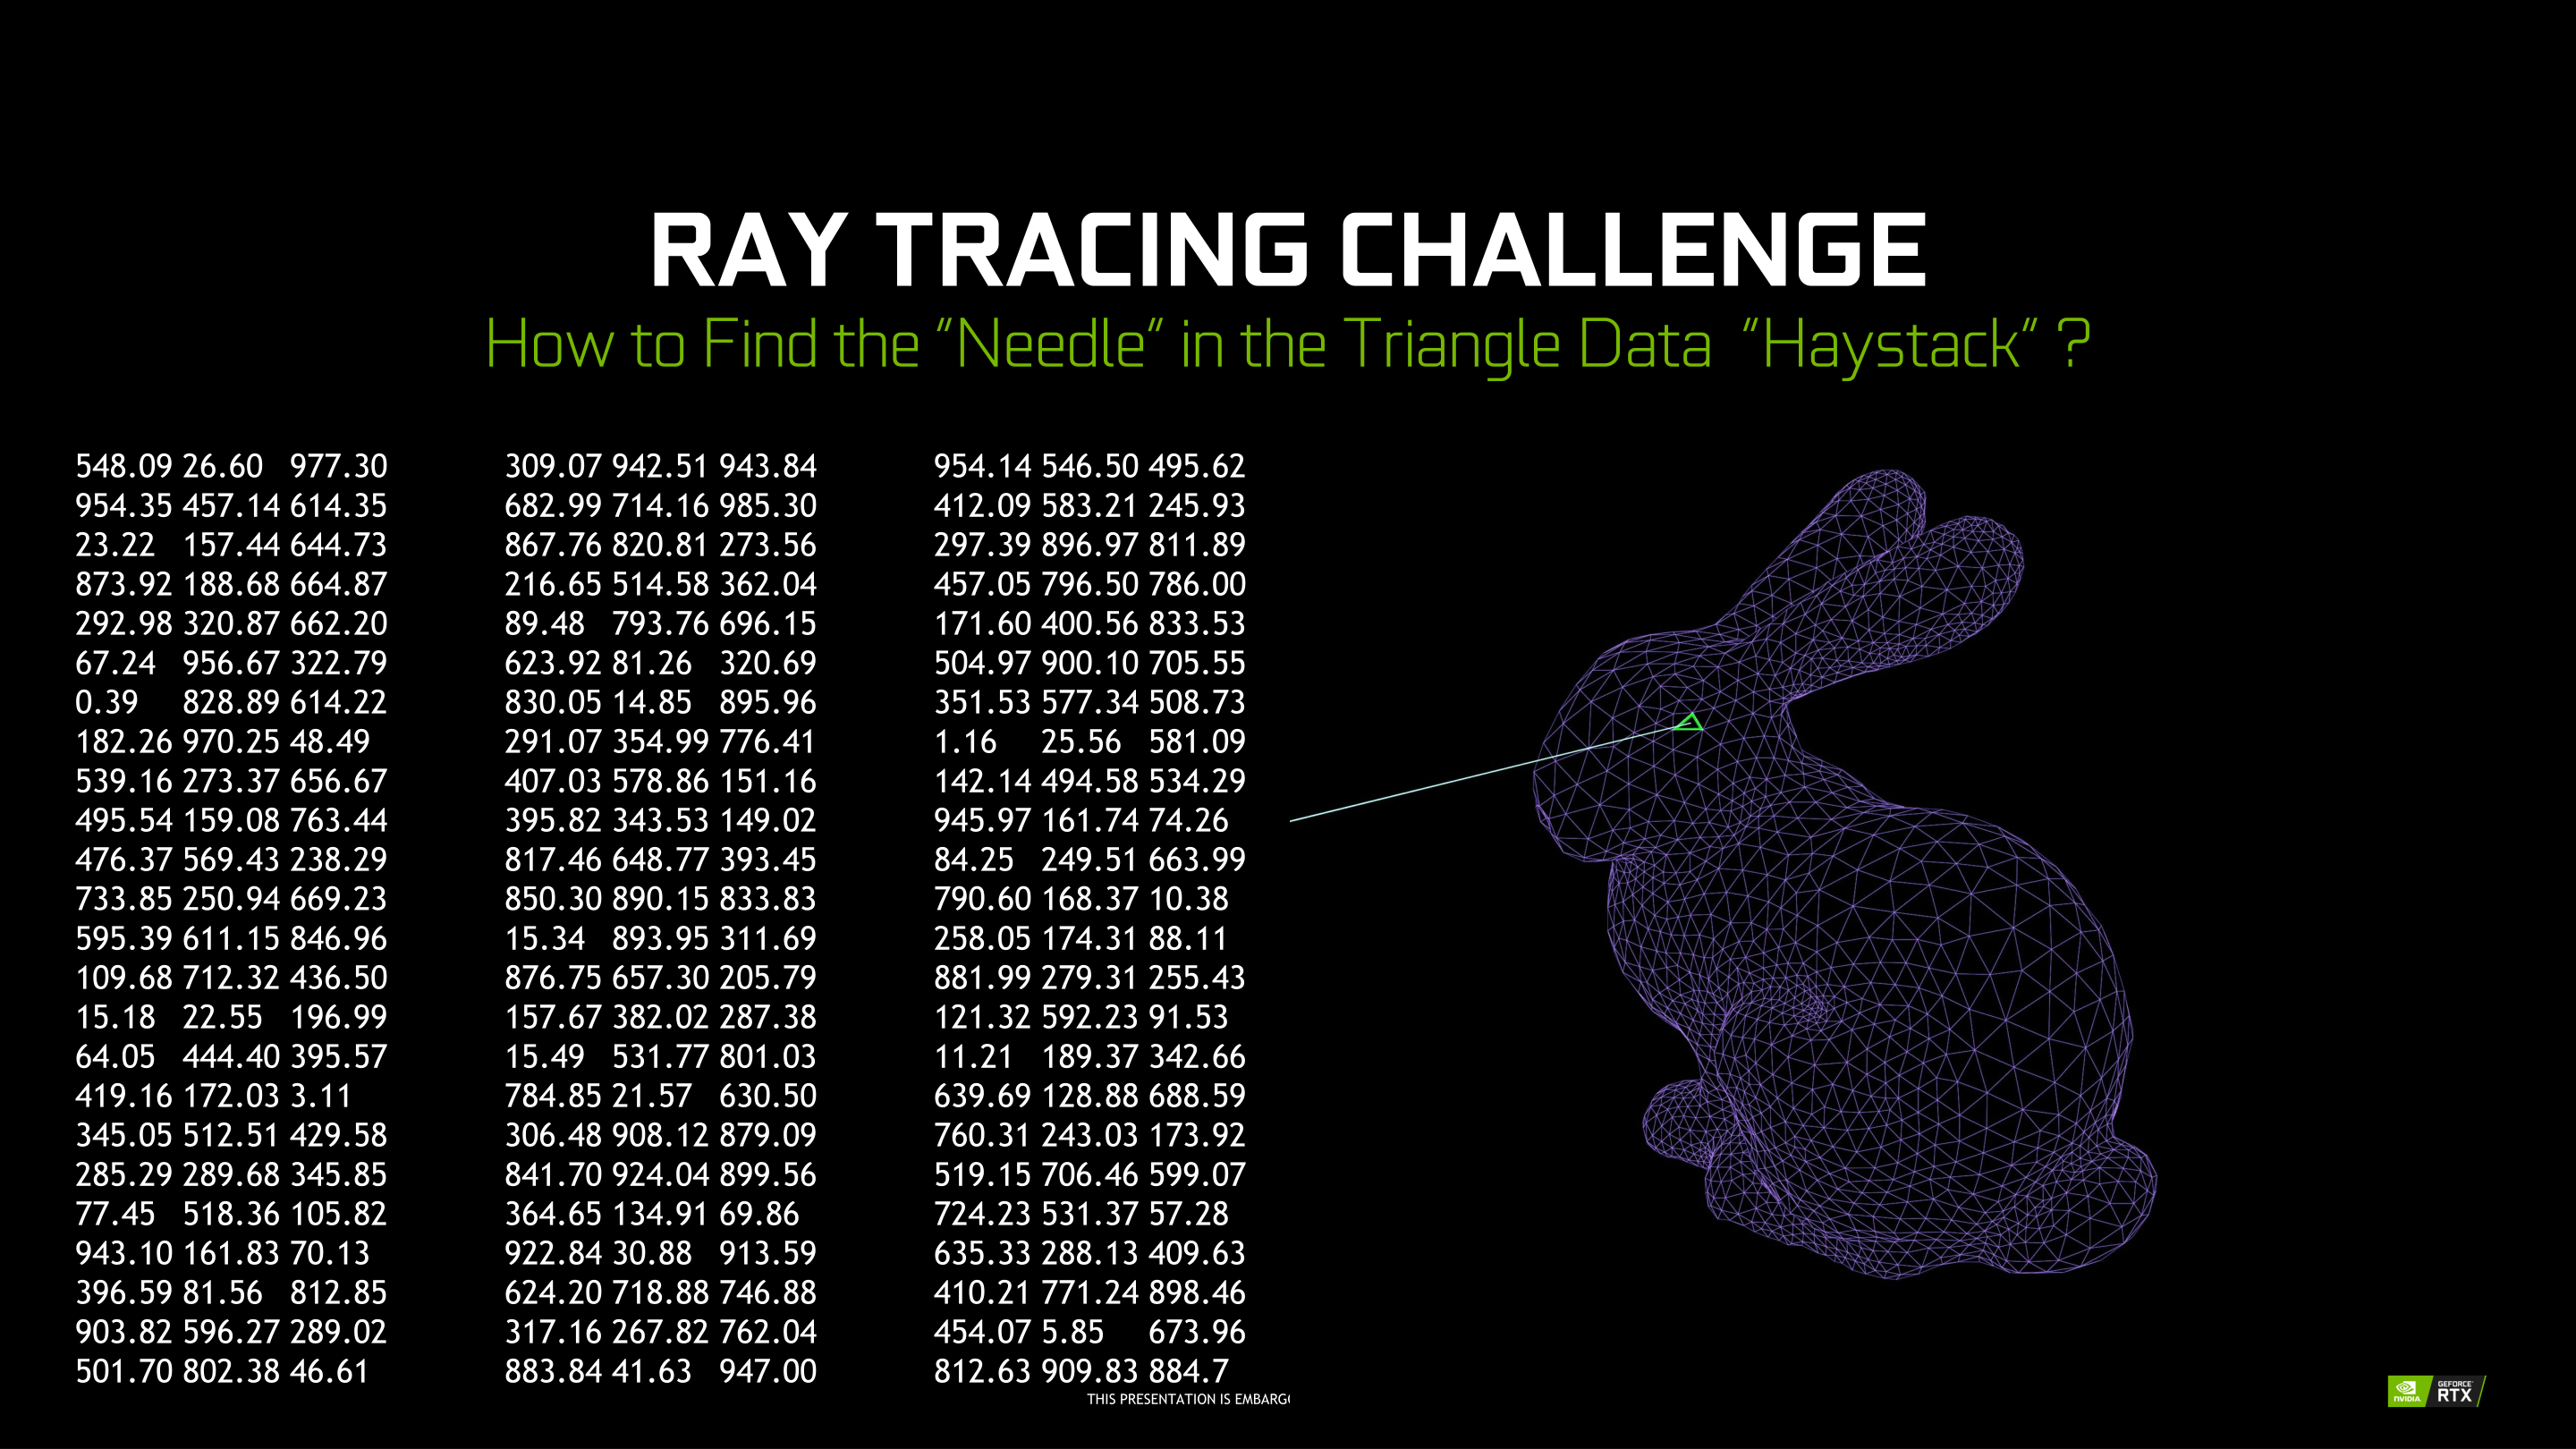
\includegraphics[width=11cm]{bilder/ray.png}
\end{frame}

\begin{frame}
	\frametitle{\phantom{}}
		\vspace{-1cm}
		\[
		\small
	\text{A} = \frac{\text{Grundseite} \times \text{Höhe}}{2}
		\] \\
		\vspace{4mm}
		\textmd{\small Wenn jedoch die Koordinaten der Eckpunkte des Dreiecks bekannt sind, kann man den Flächeninhalt mit Hilfe der sogennanten Schoelace Formela berechnen.}
		\[
		\text{A} = |\frac{(b_{x} - a_{x})(c_{y} - a_{y}) - (c_{x} - a_{x})(b_{y} - a_{y})}{2}|
		\]	
\end{frame}

\begin{frame}
	\frametitle{\phantom{}}
	\textmd{\small Wenn jedoch die Koordinaten der Eckpunkte des Dreiecks bekannt sind, kann man den Flächeninhalt mit Hilfe der sogennanten Schoelace Formel berechnen.}
	
	\[
	\text{A} = |\frac{(b_{x} - a_{x})(c_{y} - a_{y}) - (c_{x} - a_{x})(b_{y} - a_{y})}{2}|
	\]	\\
	\centering
	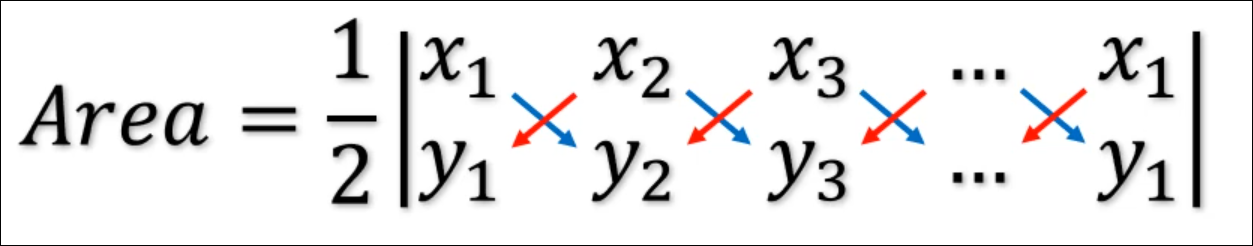
\includegraphics[width=7cm]{bilder/shoe.png}
\end{frame}

\begin{frame}
	\frametitle{\phantom{}}
	\begin{minipage}{0.6\textwidth}
		\vspace{5mm}
		\small
		Wie kommt sie zustande? \\
		\[
		\small
		\text{A} = \frac{1}{2} \left||b \times c \right|| = \frac{1}{2} \left||(B - A) \times (C - A) \right|| 
		\]
		\[
		\small =
		\frac{1}{2}
		\left| 
		\begin{matrix} 
			B_{x} - A_{x} & C_{x} - A_{x} \\
			B_{y} - A_{y} & C_{y} - A_{y}\\ 
		\end{matrix}
		\right|
		\]
		
		\[  =\frac{1}{2}
		\left| 
		\begin{matrix} 
			a_{x} & b_{x} & c_{x} \\
			a_{y} & b_{y} & c_{y} \\
			1 & 1 & 1 
		\end{matrix}
		\right|
		\]
		\[ =
		\frac{1}{2} \left( \left| 
		\begin{matrix} 
			b_{x} & c_{x} \\
			b_{y} & c_{y} \\
		\end{matrix}
		\right| 
		+
		\left| \begin{matrix}
			a_{x} & c_{x} \\
			a_{y} & c_{y}
		\end{matrix} \right|
		+
		\left| 
		\begin{matrix}
			a_{x} & b_{x} \\
			a_{y} & b_{y}
		\end{matrix}
		\right| \right) =
		\]
		\vspace{3mm}
		\[
		\frac{(b_{x}c_{y} - c_{x}b_{y}  + c_{x}a_{y} - a_{x}c_{y} + a_{x}b_{y} - a_{y}b_{x})}{2}
		\]
	\end{minipage}%
	\hfill
	\begin{minipage}{0.3\textwidth}
		\hspace{-10mm}
		\centering
		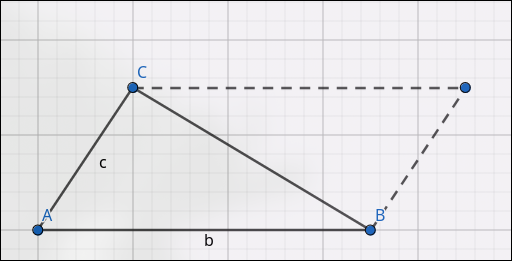
\includegraphics[width=4cm]{bilder/geo.png}
	\end{minipage}
\end{frame}

\begin{frame}
\frametitle{\phantom{}}
\small
Geometrische Darstellung
\[
\text{A} = \frac{1}{2}(b_{x} - a_{x})(c_{y} - a_{y}) - (c_{x} - a_{x})(b_{y} - a_{y})
\] \\
\centering
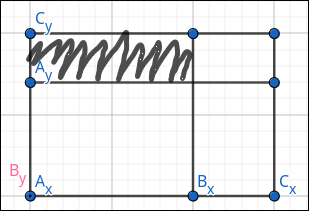
\includegraphics[width=2.5cm]{bilder/geo1.png}
\hspace{2mm}
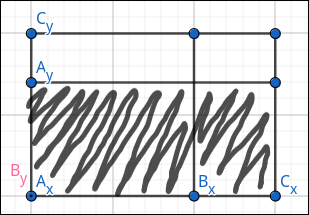
\includegraphics[width=2.5cm]{bilder/geo2.png}

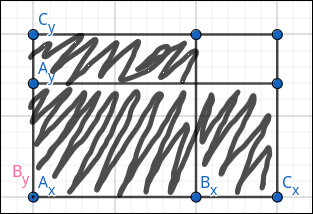
\includegraphics[width=2.5cm]{bilder/geo3.png}
\hspace{2mm}
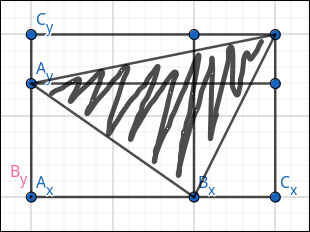
\includegraphics[width=2.5cm]{bilder/geo5.png}
\end{frame}

\begin{frame}
	\frametitle{\phantom{}}	
	\begin{figure}
		\centering
		
\includegraphics[width=8cm]{bilder/chicken.png}
	\end{figure}
\end{frame}

\begin{frame}
	\frametitle{}	
	\begin{figure}
		\centering
		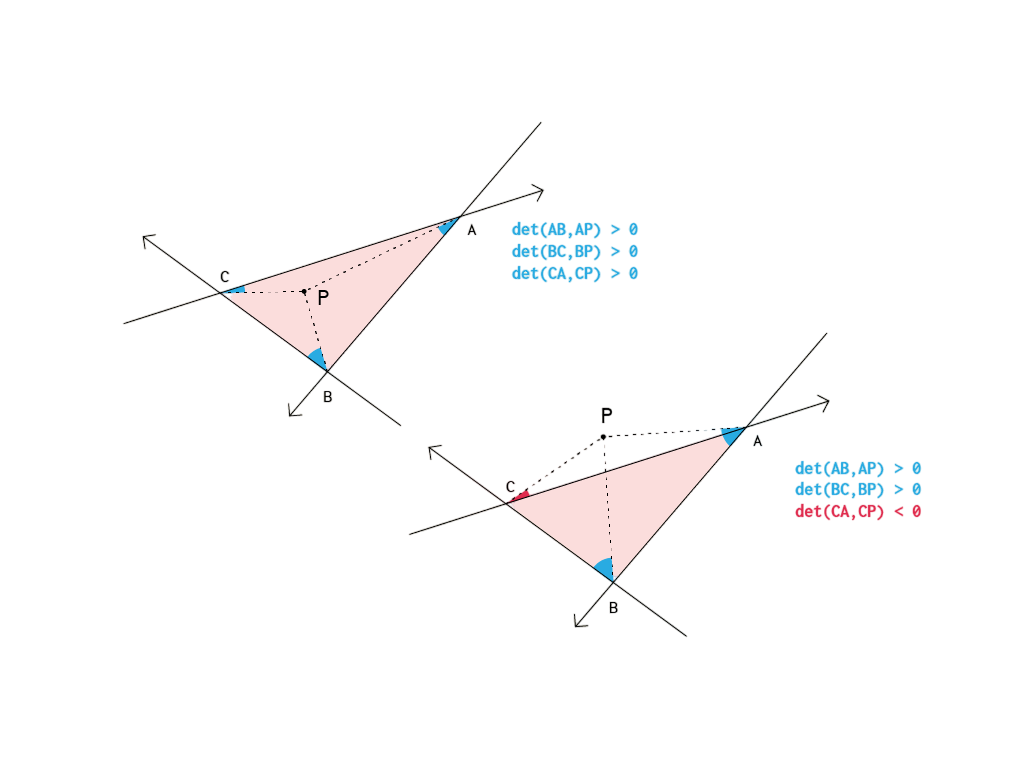
\includegraphics[width=10cm]{bilder/points-.png} 
	\end{figure}
\end{frame}

\begin{frame}
	\frametitle{\phantom{}}
	\small 
	Definition: \\
	Sei $\Omega$ ein konvexes Polygon im \(\mathbb{R}^2\), gegeben durch n Ecken $P_{1}...P_{n} n >= 3$, in CCW - Anorndnung. Eine Menge von Abbildungen  \[\lambda_{i}: \Omega \longrightarrow \mathbb{R}\] heißt baryzentrische
	Koordinaten, wenn für alle $X \in \Omega$ folegende Bedinungen gelten:
	\begin{itemize}
	\item Telung der Eins $\sum_{i=1}^{n} \lambda_{i}(X)= 1 \hspace{3mm}$
	\item Lineare Konvergenz $\sum_{i=1}^{n} \lambda_{i}(X)P_{i}= X$
	\item Konvexe Kombnation $\forall i=1...n: \lambda_{i}(X) \geq 0$
	\end{itemize}
\end{frame}
	
\begin{frame}
	\frametitle{\phantom{}}
	Wegen $\sum \lambda_{i}(X)= 1$ 
	\[\sum \lambda_{i}P_{i} = X \leftrightarrow \sum \lambda_{i}(P_{i} - X) = 0 \]
	Hat man $w_{i} = w_{i}X$ für die 
	\[\sum w_{i}(P_{i} - X) = 0 \hspace{3mm} w_{i} \geq 0\] 
	so kann  man daraus baryzentrische Koordinaten machen, indem man:
	\[\lambda_{i} = \frac{w_{i}}{\sum_{i=1}^{n} w_{i}}\] 
\end{frame}

\begin{frame}
	\frametitle{Rotation}
	\begin{minipage}{0.6\textwidth}
	\small
	Nun kann man ablesen 
	\[
	x' =
	\begin{pmatrix}
		\cos(\alpha) \\
		\sin(\alpha) \\
	\end{pmatrix}
	\quad 
	y' =
	\begin{pmatrix}
		-\sin(\alpha) \\
		\cos(\alpha) \\
	\end{pmatrix}
	\]
	Achsen jetzt in die Zeilen einer Matrix einsetzen,
	\[
	M_{rotation2D} =
	\begin{pmatrix}
		\cos(\alpha) & \sin(\alpha) \\
		-\sin(\alpha) & \cos(\alpha)
	\end{pmatrix}
	\]
	\end{minipage}
	\hfill
	\begin{minipage}{0.3\textwidth}
		\hspace{-10mm}
		\centering
		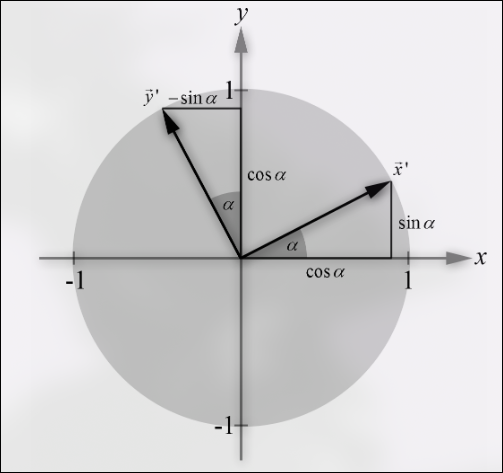
\includegraphics[width=4cm]{bilder/circle.png}
	\end{minipage}
		
	\end{frame}
	
\begin{frame}
	\frametitle{\phantom{}}
	\textmd{\small Die neuen Achsen haben immer noch die Länge 1 und
	sie sind auch senkrecht zueinander. Beides sind Merkmale einer Rotationsmatrix.} \\
	\[
\quad
\small
M_{x}
\begin{pmatrix}
	1 & 0 & 0 \\
	0 & \cos(\alpha) & \sin(\alpha) \\
	0 & -\sin(\alpha) & cos(\alpha)
\end{pmatrix}
\quad \!
\quad
M_{y}
\begin{pmatrix}
	\cos(\alpha) & 0 & \sin(\alpha) \\
	0 & 1 & 0 \\
	-sin(\alpha) & 0 & \cos(\alpha) 
\end{pmatrix}
\quad \!
\]
\[
\small
M_{z}
\begin{pmatrix}
	\cos(\alpha) & \sin(\alpha) & 0 \\
	-\sin(\alpha) & \cos(\alpha) & 0 \\
	0 & 0 & 1
\end{pmatrix}
\]
\end{frame}

\begin{frame}
	\frametitle{\phantom{}}
	\textmd{\small Möchte man um eine beliebige Achse drehen  dann kann man die unten angegebene Rotationsmatrix anwenden. Einheitsvektor $a=(a_{1},a_{2},a_{3})$ stellt die Achse dar, um die edreht werden soll: }
		\[
	\tiny
	M_{x}
	\begin{pmatrix}
		\cos(\alpha)+a_{1}^2*(1 - \cos(\alpha))  & a_{1}a_{2}(1 - \cos(\alpha)) - a_{3}\sin(\alpha)) & a_{1}a_{2}(1 - \cos(\alpha)) + a_{2}\sin(\alpha)\\
		a_{2}a_{1}(1 - \cos(\alpha)) + a_{3}\sin(\alpha)) & \cos(\alpha)+a_{2}^2*(1 - \cos(\alpha)) & a_{2}a_{3}(1 - \cos(\alpha)) + a_{1}\sin(\alpha)) \\
		a_{3}a_{1}(1 - \cos(\alpha)) - a_{2}\sin(\alpha)) & a_{3}a_{2}(1 - \cos(\alpha)) + a_{1}\sin(\alpha) & \cos(\alpha)+a_{3}^2*(1 - \cos(\alpha)) 
	\end{pmatrix}
	\]
\end{frame}

\begin{frame}
	\frametitle{Quellen}
	\begin{itemize}
		\small
		\item \href{https://www.david-scherfgen.de/downloads/neues-buch-kapitel-3d-grafik.pdf}{https://www.david-scherfgen.de/downloads/neues-buch-kapitel-3d-grafik.pdf}
		\item \href{https://cgvr.cs.uni-bremen.de/teaching/cg2_12/folien/Generalbarycentriccoords.pdf}{https://cgvr.cs.uni-bremen.de/teaching/cg212/folien/Generalbarycentriccoords.pdf}
		\item \href{https://www.scratchapixel.com/lessons/3d-basic-rendering/ray-tracing-rendering-a-triangle/barycentric-coordinates.html}{https://www.scratchapixel.com/lessons/3d-basic-rendering/ray-tracing-rendering-a-triangle/barycentric-coordinates.html}
		\item \href{https://mathoverflow.net/}{https://mathoverflow.net/}
		\item \href{https://old.mipt.ru/education/chair/mathematics/study/}{https://old.mipt.ru/education/chair/mathematics/study/}
	\end{itemize}
\end{frame}
\end{document}